\section{Time plan}
% TODO(anton):
% - Decide on suitable iterations
% - Road Genration Iteration 0: Generate mesh from bézier curve? This can be developed along side the other iterations. doesn't fit my stupid iteration model.
% - Include GANTT Chart in a more readable format
%

A time plan has been devised to aid the project in staying in phase and keeping the project realistic in relation to the time restriction of the project.
This includes time management of administrative tasks such as the project launch, the developing of the end product as well as the final report.

\subsection{Development of end product}
The three identified subproblems, described in section~\nameref{sec:problem}, facilitates a natural division of work since each of the subtasks can almost entirely be developed in isolation.
For instance the road generation can start off by only considering a strictly flat terrain.
Each subproblem is therefore further broken down into iterations so that the different systems can be developed simultaneously with as few dependency conflicts as possible.

Each iteration of a subproblem will start off as an isolated simple solution and increase in complexity and coupling with the other subsystems.
This approach will aid in working in a more cost-effective way when developing the end product.

Once all subtasks have undergone all iterations, our efforts will be targeted at fine-tuning the final solution as well as implementing as many of our stretch goals as possible.

\subsubsection{Terrain Generation}
\begin{description}
  \item[Iteration 1] Generate a simple height-map terrain mesh.
  \item[Iteration 2] Texture the terrain based on height levels.
  \item[Iteration 3] Populate the terrain with lakes, oceans and foliage.
\end{description}

\subsubsection{Road Generation}
\begin{description}
  \item[Iteration 1] Procedurally generate a convincing road-network on a 2D plane.
  \item[iteration 2] Convert the conceptual road-network into a road mesh.
  \item[Iteration 3] When generating a road from point A to point B, take the height difference in the underlying terrain into account in order to create a natural looking path.
\end{description}

\subsubsection{Building Generation}
\begin{description}
  \item[Iteration 1] Procedurally generate simple block buildings of skyscrapers, villas, terraced houses, apartments, and parks.
  \item[Iteration 2] Given a plot of land, populate it with suitably placed buildings.
\end{description}

\subsubsection{Application}
\begin{description}
  \item[Iteration 1]
    This iteration should have a working button for generating the terrain, roads, and buildings.
    The generated city should also be able to be exported to a \textit{.fbx} file.
    The quality of the generated city at this iteration is not important but rather the functionality and project skeleton to expand upon.
  \item[Iteration 2]
    The user should be able to specify parameters that affect the generated world.
    This includes parameters such as sea level and the world size.
    Also, the user should be able to place population markers using different road strategies e.g.\ Paris, Manhattan, or Chaotic.
\end{description}

\subsection{Final report}
When it comes to the final written report we are expected to continuously work on the final report during the development.
However, we have also set a three-week period strictly dedicated to finalizing the report.
At that point we expect the algorithm to be complete as to prioritize the final report.

\subsection{Project plan chart}
To get an overview of our time plan we have decided to include a GANTT chart seen in Figure~\ref{fig:time-plan} that roughly describe the expected time of the different tasks.

\newpage
\begin{figure}[H]
  \centering
  \vspace*{-1.0cm}
  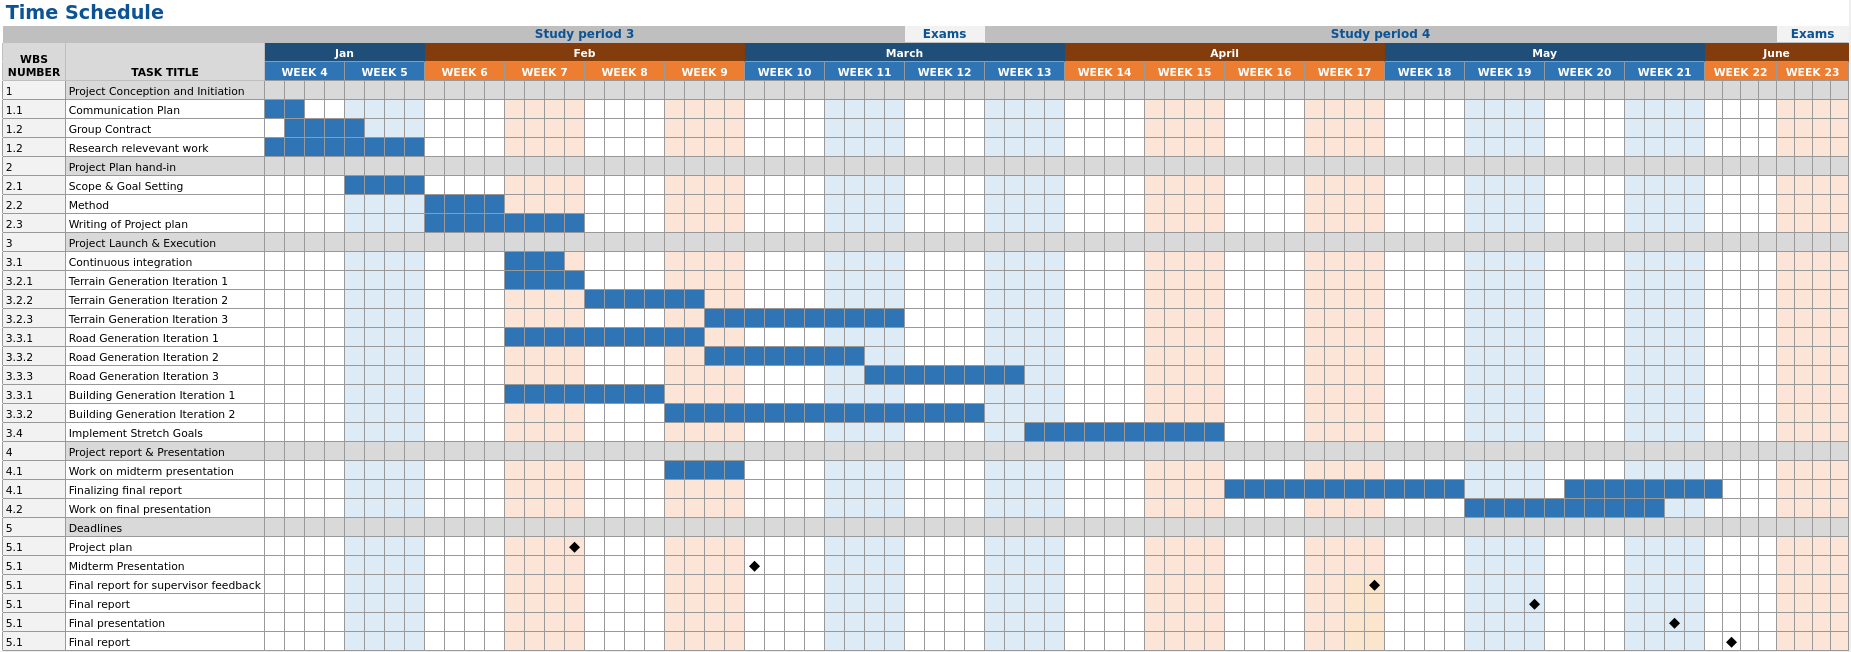
\includegraphics[angle=90, width=0.5\textwidth]{figure/time-plan.png}
  \caption{Time plan.}
  \label{fig:time-plan}
\end{figure}

